\documentclass{article} % For LaTeX2e
\usepackage{nips12submit_e,times}

\usepackage{color}
\usepackage{algpseudocode}
\usepackage{algorithm}
\usepackage{listings}
\usepackage{graphicx}
\usepackage{subcaption}
\usepackage{caption}

\definecolor{javared}{rgb}{0.6,0,0} % for strings
\definecolor{javagreen}{rgb}{0.25,0.5,0.35} % comments
\definecolor{javapurple}{rgb}{0.5,0,0.35} % keywords
\definecolor{javadocblue}{rgb}{0.25,0.35,0.75} % javadoc
% "define" Scala
\lstdefinelanguage{scala}{morekeywords={class,object,trait,extends,with,new,if,while,for,def,val,var,this},
otherkeywords={->,=>},
sensitive=true,
morecomment=[l]{//},
morecomment=[s]{/*}{*/},
morestring=[b]"}
% Default settings for code listings
\lstset{frame=tb,language=scala,aboveskip=3mm,belowskip=3mm,showstringspaces=false,columns=flexible,basicstyle={\small\ttfamily},
keywordstyle=\color{javapurple}\bfseries,
stringstyle=\color{javared},
commentstyle=\color{javagreen},
morecomment=[s][\color{javadocblue}]{/**}{*/}}
%\documentstyle[nips12submit_09,times,art10]{article} % For LaTeX 2.09


\title{A Comparison of Parallel Algorithms:\\ {\Large Hogwild!, Shotgun and Distributed Averaging}}

\author{
David A. Leen \\
Department of Applied Mathematics\\
University of Washington \\
\texttt{dleen@uw.edu} \\
\And
Brian D. Walker \\
Department of Computer Science \& Engineering \\
University of Washington \\
\texttt{walker7734@gmail.com} \\
}

% The \author macro works with any number of authors. There are two commands
% used to separate the names and addresses of multiple authors: \And and \AND.
%
% Using \And between authors leaves it to \LaTeX{} to determine where to break
% the lines. Using \AND forces a linebreak at that point. So, if \LaTeX{}
% puts 3 of 4 authors names on the first line, and the last on the second
% line, try using \AND instead of \And before the third author name.

\newcommand{\fix}{\marginpar{FIX}}
\newcommand{\new}{\marginpar{NEW}}

\nipsfinalcopy % Uncomment for camera-ready version

\begin{document}
\maketitle

\begin{abstract}
We implemented the Hogwild! algorithm and demonstrated an approximately linear speedup over the
sequential stochastic gradient descent (SGD) algorithm.  We used the click prediction dataset and its sparse search token features to test the algorithms. We implement and demonstrate the close to optimal speedup of the Distributed Averaging method. Several strategies are detailed for dealing with mixed-sparsity data i.e. data that has both sparse and dense components. We implement a potentially novel combination of Hogwild!~and Distributed Averaging. We demonstrate the favorable trade-off between speedup and test error that this method gives on mixed-sparsity data. We finally test these algorithms on some synthetic data derived from the click prediction data set, where the number of dense user features and sparse tokens is increased.
\end{abstract}

\section{Introduction}
We study three parallel algorithms: Hogwild! \cite{niu2011hogwild}, Shotgun \cite{bradley2011parallel} and distributed averaging \cite{zhang2012comunication}. Each approaches a similar problem in a distinct manner. Hogwild! and distributed averaging parallelize stochastic gradient descent (SGD) over samples, whereas Shotgun tackles the orthogonal problem of parallelizing $L_1$-regularized models over the features.

Hogwild!~is just one particular realization of parallel SGD \cite{niu2011hogwild, zinkevich2010parallelized}. The algorithm is intended for problems on the order of several terabytes of data. It can be run quite effectively on inexpensive multi-core systems taking advantage of the low latency and high throughput of the data being stored in RAM or a RAID disk setup close to the processors. In these systems the bottlenecks arise from synchronizing and locking operations on the threads reading and writing shared memory. Regularization can also be applied in parallel settings \cite{langford2009slow, agarwal2011distributed}.

MapReduce in contrast deals with hundreds and thousands of terabytes of data but is not well suited for online, iterative algorithms like SGD. MapReduce suffers from low throughputs due to fault tolerance and redundancy. Distributed averaging is a simple version of a distributed optimization algorithm \cite{dekel2012optimal, agarwal2011distributed}. The method distributes the data samples evenly in group to some number of machines. Each machine performs a separate minimization of each group independently of one another. The estimates of the weights from each group are then averaged hence the name.

Shotgun provides a parallel solution to the high-dimensional problem with a large number of features using $L_1$-regularization \cite{ng2004feature}. In cases like this the dimensionality of the problem often dwarfs the number of samples. Once again the method involves taking a sequential algorithm, coordinate descent and simply parallelizes it, this time over features. The algorithm makes the coordinate updates in parallel to provide a speedup.

We study these algorithms in the context of the click prediction dataset. We first briefly discuss the algorithms, the challenges associated with parallel programming, then specific challenges associated with the click prediction dataset. Finally we present our results and our ``replicate'' strategy for mixed-sparsity data.

\section{Method}
The weight vector $w$ for logistic regression is updated according to the usual SGD equation:
\begin{equation}
w_i^{t+1} \leftarrow w_i^t + \eta \bigg[y^t - \frac{\exp{(w^t \cdot x^t)}}{1 + \exp{(w^t \cdot x^t)}} \bigg]x_i^t.
\end{equation}

\subsection{Proof of concept}
The minimal example demonstrating the Hogwild! concept in practice for a simple mapping is (in Scala for brevity):
\begin{lstlisting}
val weights = collection.mutable.Map[Int, Double]() // create a mapping
for (i <- data.keys) weights.put(i, 0.0) // initialize key values to 0.0
for (k <- samples.par, i <- feature.keys) weights(i) += gradient // update
\end{lstlisting}
This parallel version of SGD (using the \verb+.par+ method) produces non-deterministic values for the weights as expected. This is due to a race condition caused by threads overwriting one another. The Hogwild! algorithm relies on the sparsity of the data to ensure that updates do not operate simultaneously on the same keys. It relies on the same sparsity to parallelize the sequential algorithm.

\subsection{Algorithm}

\begin{algorithm}
  \caption{Hogwild! update step for a single processor}

  \begin{algorithmic}
  \Loop
  \State Randomly permute data
  \State Read current state of features $x^t$
  \For {i in $x^t$.keys}
  \State $w^{t+1}_i \leftarrow w_i^t - \eta x_i^t \nabla L(\mathbf{w}, \mathbf{x}, \mathbf{y})$
  \EndFor
  \EndLoop
  \end{algorithmic}
  \label{alg1}
\end{algorithm}

The component wise addition of elements from the weight vector is assumed to be atomic. In practice floats are not atomic and require extra care. See section \ref{gen_inst}.

\section{Challenges and issues}
\label{gen_inst}
\subsection{Parallel and concurrent programming}
Parallel programming is hard. The Hogwild!~solution is to ignore all the major issues associated with parallelism. The Hogwild!~paper discusses a compromise between full synchronization and no locking at all which they call AIG. AIG puts a lock on only the elements that are being updated inside the for loop in algorithm \ref{alg1}. This is essentially what ConcurrentHashMap in Java does. It often can be difficult to determine which regime we are operating in without resorting to a closer-to-the-hardware language like C.

Distributed Averaging takes the opposite approach avoiding the issues of parallelism altogether. It turns the problem into a data parallel one by dividing the data into a number of chunks, one per machine or processor and running SGD in parallel on each one independent of the others. The weights are then averaged. 

\subsection{Storing data in memory}
The Hogwild!~algorithm relies on extremely fast throughput of data from memory or disk. Reading from disk is not fast enough to supply data as needed by a 4-6 core machine. This could be possible with a RAID setup but at the time this was not available. The Hogwild!~paper uses sophisticated caching and memory management to process terabyte sized data on a single machine.

Our current solution is to load and parse all the data into RAM. 8--16GB of RAM is fairly standard these days, which is sufficient for the click prediction set, but it is not enough for terabyte data sets. We need to investigate how to break data sets into manageable chunks while still sampling uniformly as needed by the algorithms. 

\subsection{Non-sparse data}
An immediate issue was whether Hogwild! can work efficiently on data with sparse and non-sparse components? The click prediction data has several dense values including age and gender. They are updated on every iteration. The tokens however are very sparse. Can we apply the Hogwild! algorithm in this case without ignoring the dense data? This issue is answered in the next section.

\section{Mixed-sparsity data}
The click prediction data provides an interesting scenario in which to test Hogwild! The click prediction dataset is comprised of user features and sparse tokens. We call this combination of sparse and non-sparse data ``mixed-sparsity''. We initially pretend the data is sparse and run Hogwild!~ before discussing strategies for improving the error while maintaining the speedup from the extra processors.

\subsection{Strategies for mixed-sparsity data}
We outline several strategies that we implement and test on the click prediction dataset:
\begin{enumerate}
\item Locking
\item Normal
\item Random
\item Single thread
\item Replicate
\end{enumerate}

\section{Results}
Initial results ranging from one to four CPU cores. During each run the same number of updates over the data occurs with the workload evenly distributed across each core. We fall slightly short of the optimal speedup of four, figure \ref{res}(a). The Hogwild! algorithm has a slightly worse RMSE as expected, figure \ref{res}(b).
\begin{figure}[htb]
\centering
\begin{subfigure}{0.49\textwidth}
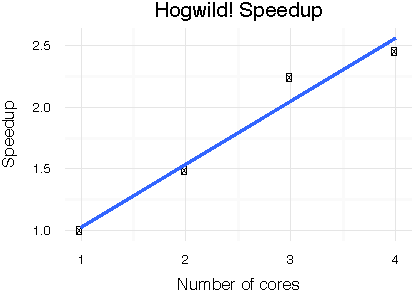
\includegraphics[width=\textwidth]{./speedup.pdf}
\end{subfigure}
\centering
\begin{subfigure}{0.49\textwidth}
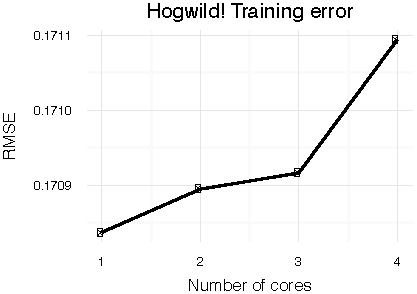
\includegraphics[width=\textwidth]{./error.pdf}
\end{subfigure}
\caption{(a) The observed speedup from experiment. The speedup with four processors is approximately 2.55.~(b) The observed root mean squared error growth with number of cores from experiment.}
\label{res}
\end{figure}
\section{Further work}
The next step is to implement Shotgun and distributed averaging for (sparse) logistic regression. We will compare all three and confirm where each performs optimally. We have the baseline sequential predictions for each data set against which we can judge speedup, convergence and error rates. We will then expand to linear regression and support vector machines and time permitting matrix completions. The data sets will be expanded from click prediction. We will continue to investigate the issue of non-sparse data contaminating the Hogwild! algorithm and whether one can perform (delayed) regularization during Hogwild!

\begin{figure}[htb]
\centering
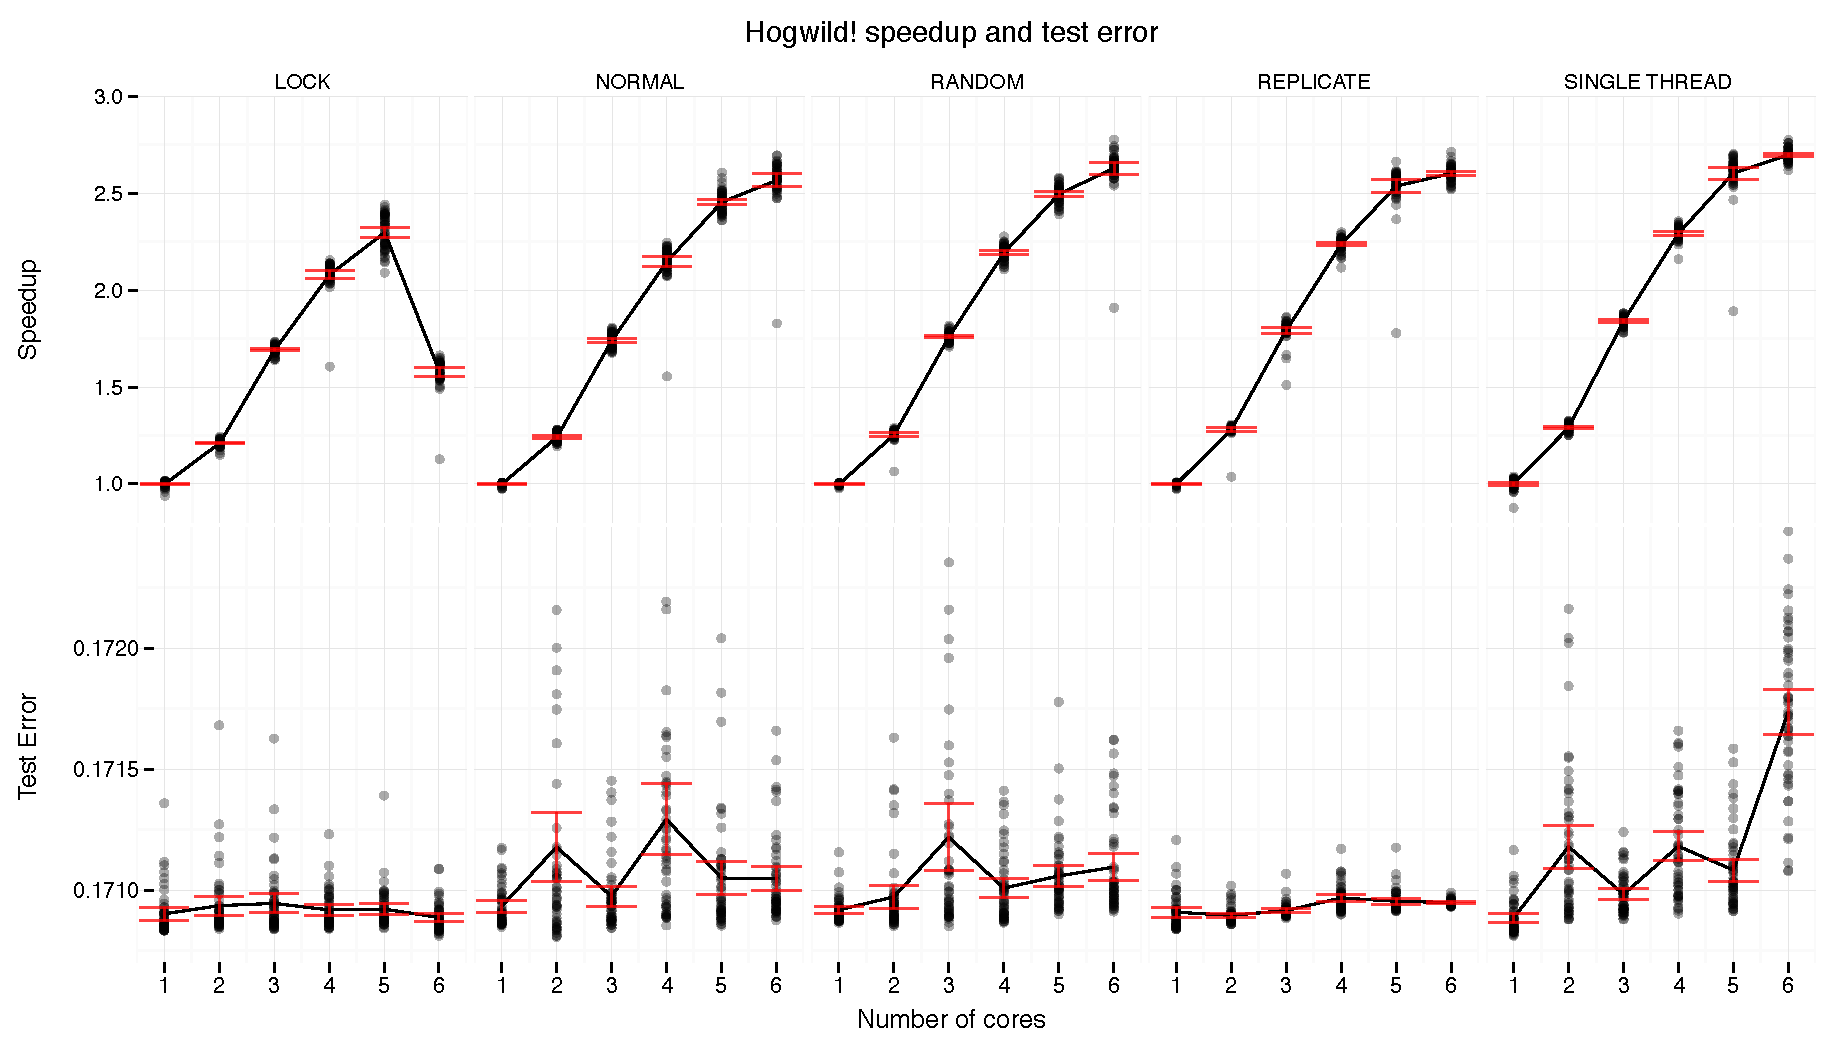
\includegraphics[width=\textwidth]{../../speedup_errors_complete.pdf}
\caption{(a) The observed speedup from experiment. The speedup with four processors is approximately 2.55.~(b) The observed root mean squared error growth with number of cores from experiment.}
\label{res}
\end{figure}

\begin{figure}[htb]
\centering
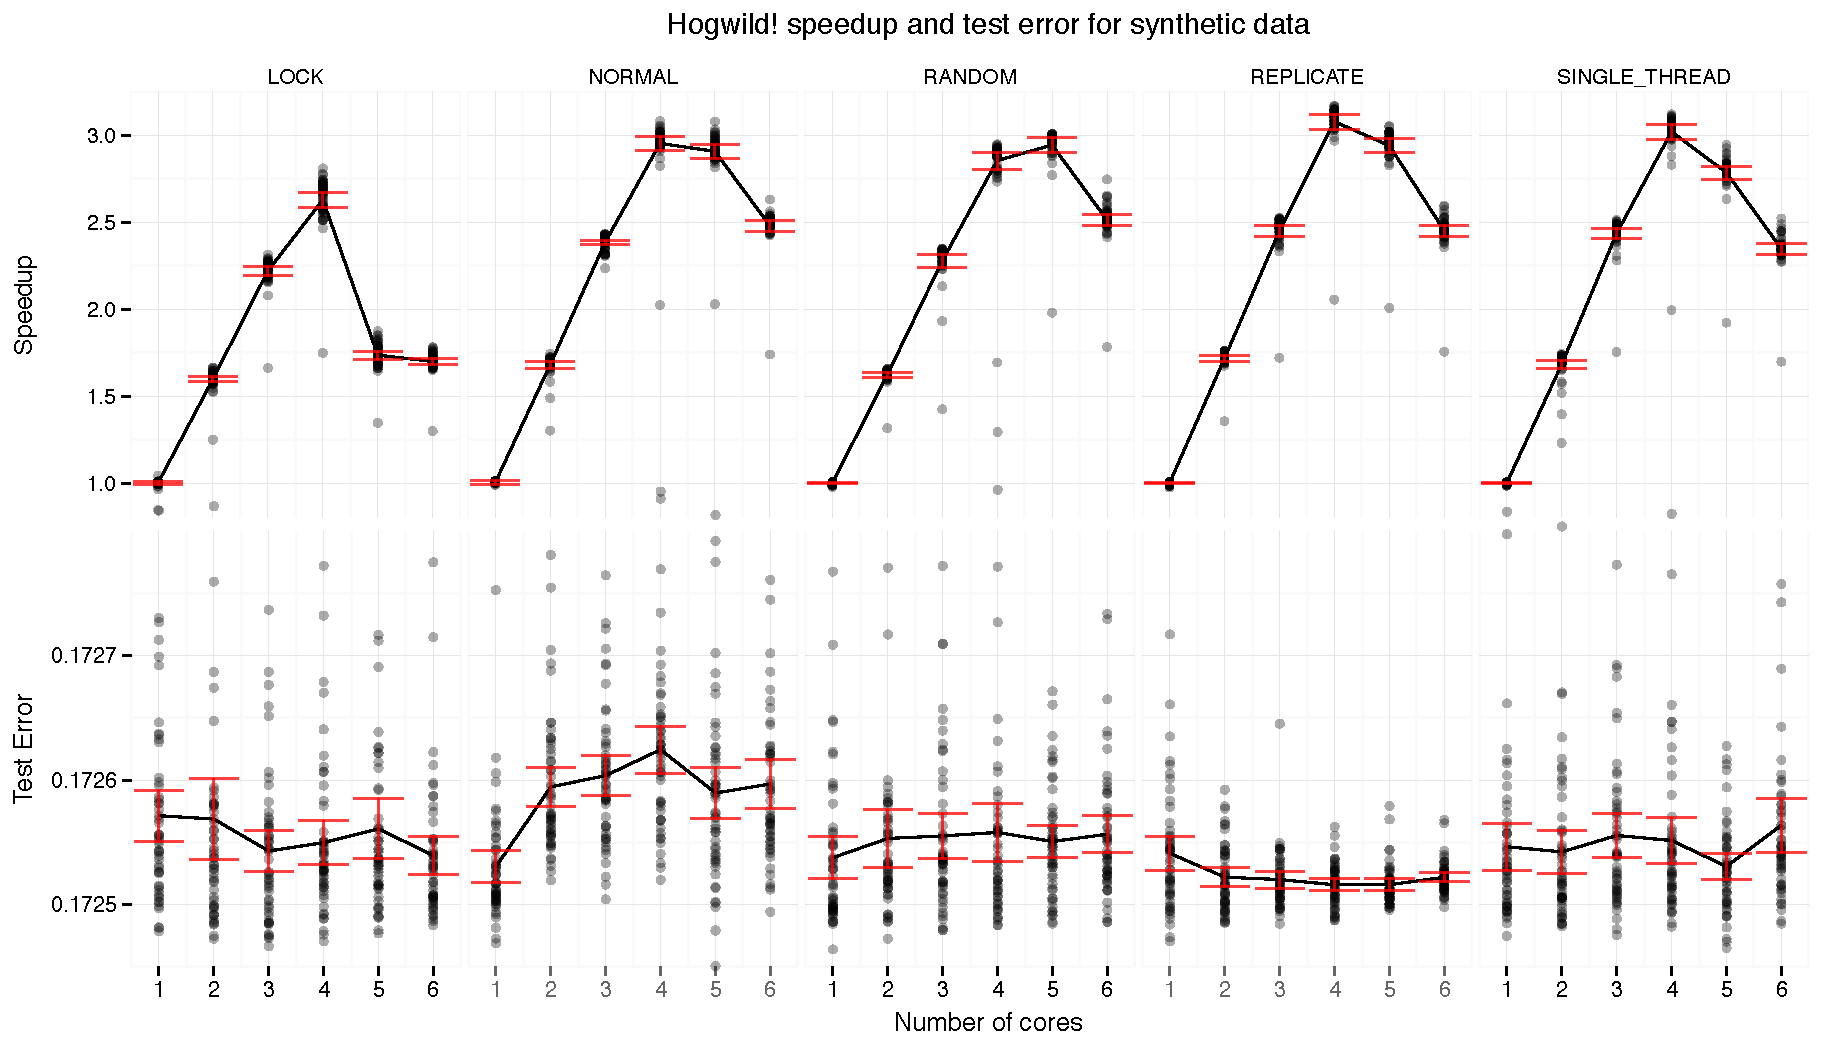
\includegraphics[width=\textwidth]{../../speedup_errors_complete_syn.pdf}
\caption{(a) The observed speedup from experiment. The speedup with four processors is approximately 2.55.~(b) The observed root mean squared error growth with number of cores from experiment.}
\label{res}
\end{figure}

\begin{figure}[htb]
\centering
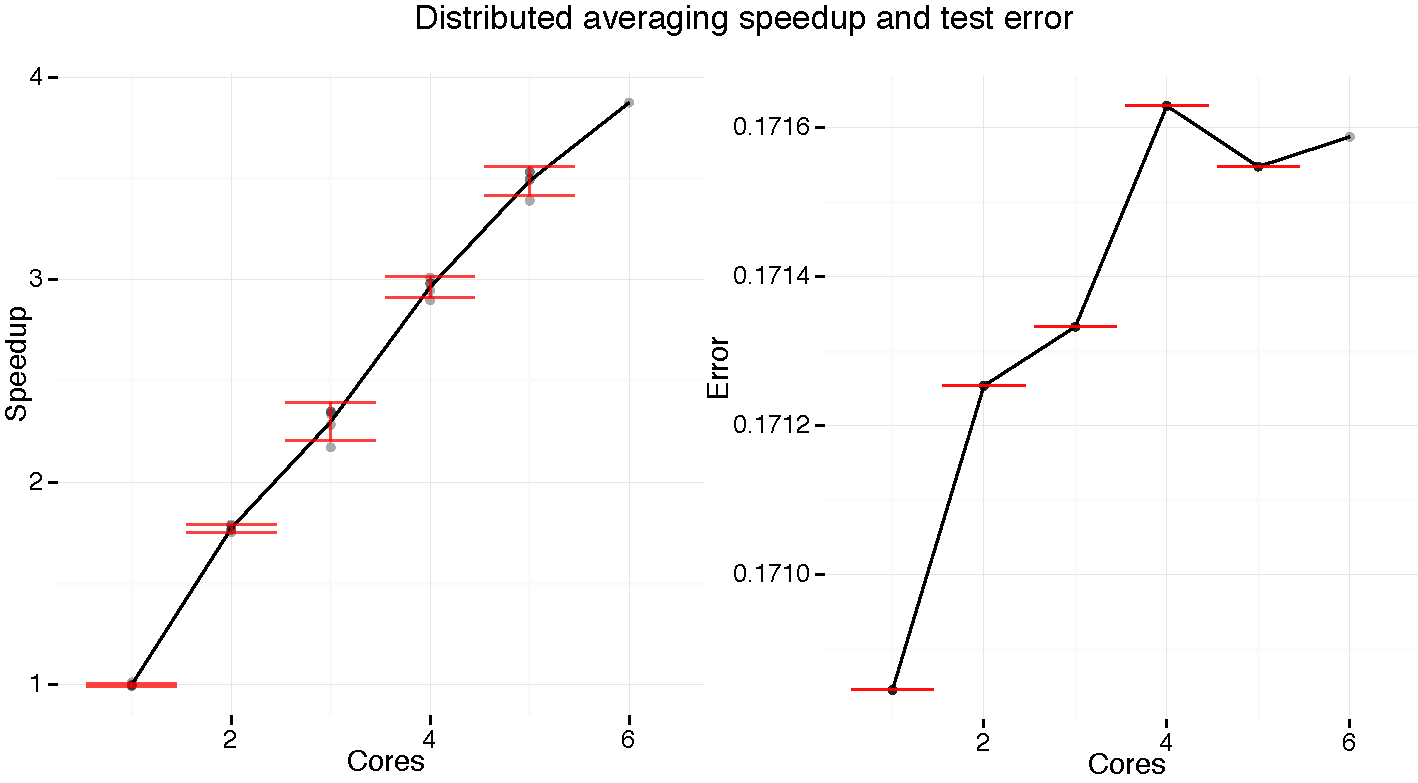
\includegraphics[width=0.8\textwidth]{../../dist_avg.pdf}
\caption{(a) The observed speedup from experiment. The speedup with four processors is approximately 2.55.~(b) The observed root mean squared error growth with number of cores from experiment.}
\label{res}
\end{figure}

\section{To Do List}
\begin{enumerate}
\item Discuss theory behind averaging. When will it work?
\item Theory behind Hogwild.
\end{enumerate}


\subsubsection*{References}

\begingroup
\renewcommand{\section}[2]{}%
%\renewcommand{\chapter}[2]{}% for other classes
\bibliographystyle{unsrt}
\bibliography{references}
\endgroup


\end{document}
